\documentclass[12pt]{article}
\usepackage{graphicx}
\setlength{\textwidth}{6.5in}
\setlength{\textheight}{9.0in}
\setlength{\topmargin}{-0.6in}
\setlength{\oddsidemargin}{0.0in}
\setlength{\evensidemargin}{0.0in}
\begin{document}
\graphicspath{{figs/}}

\vspace*{\fill}
\begin{center}
{\Large \bf  
CLUSTER: An Unsupervised Algorithm \\
for Modeling Gaussian Mixtures}\\
\bigskip
{\em Charles A. Bouman}\\
School of Electrical Engineering\\
Purdue University\\
West Lafayette IN 47906\\
bouman@ecn.purdue.edu\\
(765) 494-0340\\
http://www.ece.purdue.edu/\verb|~|bouman\\
Version 2 - April 1997\\
Version 3 - September 1998\\
Version 3.2 - December 1999; May 2000 - manpage update\\
Version 3.3 - September 2000 - manpage update\\
Version 3.4 - October 2001 - manpage update\\
Version 3.6.4 - July 2005 - manpage update\\
\end{center}

\section*{Developed by:}

\hspace*{0.5in}
\parbox{6in}{
\noindent
Charles A. Bouman; School of ECE, Purdue University\newline
Michael Shapiro; NCSA\newline
Gregory W. Cook; School of ECE, Purdue University\newline
C. Brian Atkins; School of ECE, Purdue University\newline
Hui Cheng; School of ECE, Purdue University\newline
Jennifer G. Dy; School of ECE, Purdue University\newline
Sean Borman; Department of Electrical Engineering, University of Notre Dame\newline
}

\vspace*{\fill}

{\footnotesize
\noindent
Copyright (c) 1995 The Board of Trustees of Purdue University.

Permission to use, copy, modify, and distribute this software and its
documentation for any purpose, without fee, and without written agreement is
hereby granted, provided that the above copyright notice and the following
two paragraphs appear in all copies of this software.

In no event shall Purdue University be liable to any party for direct,
indirect, special, incidental, or consequential damages arising out of the
use of this software and its documentation, even if Purdue University has
been advised of the possibility of such damage.

Purdue University specifically disclaims any warranties, including, but not
limited to, the implied warranties of merchantability and fitness for a
particular purpose.  The software provided hereunder is on an ``as is'' basis,
and Purdue Univeristy has no obligation to provide maintenance, support,
updates, enhancements, or modifications.
}



\newpage
\tableofcontents
\vspace*{\fill}


\newpage
\section{Introduction}

The Cluster software package is used to automatically estimate
the parameters of a Gaussian mixture model from sample
data.
This process is essentially similar to conventional clustering
except that it allows cluster parameters to be 
accurately estimated even when the clusters overlap
substantially.
The resulting mixture model is useful for a variety
of applications including texture and multispectral
image segmentation (see the SMAP segmentation
package.)

The ``clust'' program applies the expectation-maximization
(EM) algorithm together with an agglomerative clustering
strategy to estimate the number of clusters which best
fit the data.
The estimation is based on the Rissenen order
identification criteria known as minimum discription length (MDL).
This is equivalent to maximum-likelihood (ML) estimation when
the number of clusters is fixed, but in addition it allows the number
of clusters to be accurately estimated.

The package also includes two addition programs which make
``clust'' more useful.
The program ``classify'' can be used to perform maximum likelihood
classification from the parameter files generated by ``clust'',
and the program ``SplitClasses'' can be used along with ``clust'' 
and ``classify'' to perform unsupervised classification.

The software package is written in ANSI-C and is set
up to compile on a wide variety of unix platforms.
The main file directory contains the following subdirectories.

\begin{itemize}

\item[]{\bf documentation} - This subdirectory
contains this manual and other documentation.

\item[]{\bf example1} - 
Example showing how to run ``clust'' program.
This subdirectory contains a shell script that runs a simple
example showing how the "clust" program can be used
to estimate the parameters of a Gaussian mixture model
from training data.

\item[]{\bf example2} - 
Example showing how to use the ``cluster'' and ``classify''
programs together to classify vectors.
This subdirectory contains a shell script that first runs
the ``cluster'' to estimate two Gaussian mixture models (GMM).
It then runs the ``classify'' program to perform maximum
likelihood classification of vectors from the
two GMM distributions.

\item[]{\bf example3} - 
Example showing how to use the ``clust'', ``classify'', and ``SplitClasses''
to perform unsupervised classification of data vectors.
First ``clust'' forms a GMM. Next "SplitClasses" separates each component
of the GMM into a separate class. Finally, ``classify'' is used to classify
the original training vectors.

\item[]{\bf Makefile} - This makefile constructs the compiled binaries.
These makefiles have been tested for the gcc compiler under linux,
but it should also work with little or no modification on other platforms
supporting ANSI-C code. 

\item[]{\bf src} - This subdirectory contains the ANSI-C source
code and header files required for the ``clust'' program and library.

\end{itemize}




\section{Demo}
\label{sec:demo}

The Cluster software package contains 
a number of simple demos which illustrate its use.
To run these examples, simply execute the shell script
\mbox{``exampleN/Demo''} where ``N'' corresponds
to the demo number.
If you are using MS Windows, then you can just read
the contents of the demo files, and type in the commands
manually. 
In some cases, the demo files contain matlab commands
that are commented out. 
People with Matlab can use the included Matlab commands,
and associated Matlab scripts, to perform additional functions;
but everything in the package runs without Matlab.

\subsection{example1 - GMM Parameter Estimation}

This example shows how to use the program ``clust'' 
to cluster data vectors by estimating the parameters
of a Gaussian mixture model. 
The program extracts mixture model
parameters for the sample vectors contained in the file ``data''.
The demo runs four examples, and the GMM parameters
resulting from these examples are stored in the four output files
listed below:
\begin{itemize}
\item[] {\bf params} - This file is the default method which 
estimates the number of clusters using the MDL method
and uses full covariance matrix for each cluster.
\item[] {\bf params\_full5} - This method generates a user
specified number of clusters (i.e. 5) and a full covariance matrix for each cluster.
\item[] {\bf params\_diag} - This method estimates the number 
of clusters using the MDL method
and uses a diagonal covariance matrix for each cluster.
This option is useful when the amount of training data is limited.
\item[] {\bf params\_diag5} - This method generates a user
specified number of clusters (i.e. 5) 
and uses a diagonal covariance matrix for each cluster.
This option is useful when the amount of training data is limited.
\end{itemize}
All parameter files are ASCII and human readable.
The specific formate of the output files is
discussed in section \ref{sec:params_file}.

The demo can also generate new sample data using matlab.
To do this, simply run the m-file ``mk\_data.m''.

\subsection{example2 - ML Classification using GMM Models}

This example shows how the ``classify'' program 
can be used to classify test vectors into classes
where each class is model with a GMM distribution.
To do this, we first run ``clust'' to estimate the GMM
parameters for two different training sets, 
e.g. one GMM model for each class.
The parameters for each of the two GMM's are stored
in a single parameters file. 
By viewing the ``params'' file in a text editor,
you can see that the parameters for each class
are stored in a structure starting with the words ``class''
and ending with the words ``endclass''.

Once the GMM parameters are estimated for each class,
they are passed to the ``classify'' program.
The ``classify'' program performs ML classification
of test vectors using these two GMM classes.
The ``classify'' program is easy to modify 
by any experienced C programmer, so you can
incorportate the classifier into your own programs.

\subsection{example3 - Unsupervised Clustering}

This example shows how the Cluster package
can be used to perform unsupervised clustering
of data vectors.
First, a GMM model is extracted from the data
vectors using the ``clust'' algorithm.
This produces a parameter file with a single class.
However, this class typically contains a number
of multivariate Gaussian components.
Each of these components is designated in the parameter
file by ``subclass'' and ``endsubclass''.
The ``SplitClasses'' program reads in the parameter
file, separates each subclass into its own
individual class, and stores the resulting
parameter file.
Once this is done, the ``classify'' program
can be used to classify the vectors into each subcluster.
This results in unsupervised clustering of the data vectors.

\section{Clustering}
\label{sec:training}

The {\em clust} program is designed to process $M$
distinct data sets in a single pass.
The program will extract a mixture model for each data
set and store the $M$ mixture models in a signal parameter
file.
This is usefull for applications such as segmentation
when each mixture model represents one of $M$ distinct
classes that must be modeled.

In order to run the clust algorithm 
a data file must be created for each of the $M$ data sets.
Each data file contains a series of vectors 
in ASCII floating point format and on separate lines.
Each vector should be a sample from the multivariate
distribution of interest.
The clust program will use these data vectors to estimate
a Gaussian mixture model that best fits the sample data
in the corresponding file.
The Gaussian mixture model is formed by adding together
multivariate Gaussian distributions each with different
mean and covariance.
Each of these component component distributions is a cluster
(or subclass) of the distribution.

After a Gaussian mixture model has been extracted for
each data set,
the {\em clust} program will then generate a params file which contains 
all the parameters of all $M$ Gaussian mixture distributions.
Section \ref{sec:params_file} contains information
on the contents of the parameter file.

The specifics of the algorithm are described 
in Appendix~\ref{sec:parameter_est};
however, Fig.~\ref{fig:SigSet_flow_dia} illustrates the basic operations
performed in the {\em clust} program. 
The algorithm is started by initializing
with a set of cluster parameters and a user selected number of clusters.
The cluster means are generated by selecting the appropriate number of samples
from the training data, and the cluster covariances are set to all be
equal to the covariance of the complete data set.
After this initialization, 
the algorithm enters a loop in which clusters are combined
(or eliminated when empty) until only one cluster remains.

Figs.~\ref{fig:SigSet_scat_plot} 
and \ref{fig:SigSet_output} and Table~\ref{tbl:mix_params}
show the results of a simple experiment using the Cluster algorithm.
(This experiment is included as an example with the package.
You may run this example by executing the ``example/Demo'' file.)
Figs.~\ref{fig:SigSet_scat_plot} shows a scatter plot of 500 samples 
from a two dimensional random vector.
The random vector is chosen to have a distribution formed by the mixture
of three bi-variate Gaussian distributions. 
Each component of the mixture distribution, or cluster,
is parameterized by its relative proportion, $\pi_i$, its mean, $\mu_i$, 
and its covariance, $R_i$. 
The values used to generate the data are show in Table~\ref{tbl:mix_params}.
Notice, that the scatter plot has two distinct clusters, but the second
and third clusters overlap and are less distinct.

The output of the Cluster program is shown in Fig.~\ref{fig:SigSet_output}.
After two clusters are combined, the parameters for the new set
of clusters is estimated, and the final value of the MDL 
(Rissanen criteria) is printed.
Notice that the minimum of the criteria occurs at 3,
which, in this case, is the correct number clusters.
The estimated cluster parameters are listed 
in Fig.~\ref{tbl:mix_params} and the corresponding 
mixture pdf is shown in Fig.~\ref{fig:mix_pdf}.
Notice that for this data set, 
the match between the true and estimated parameters 
is reasonably close.

Refer to Appendix~\ref{sec:parameter_est} for more
details on how the {\em clust} algorithm works,
and Section~\ref{sec:C_manual} for details
on how to run the {\em clust} program.


\begin{figure}
\centerline{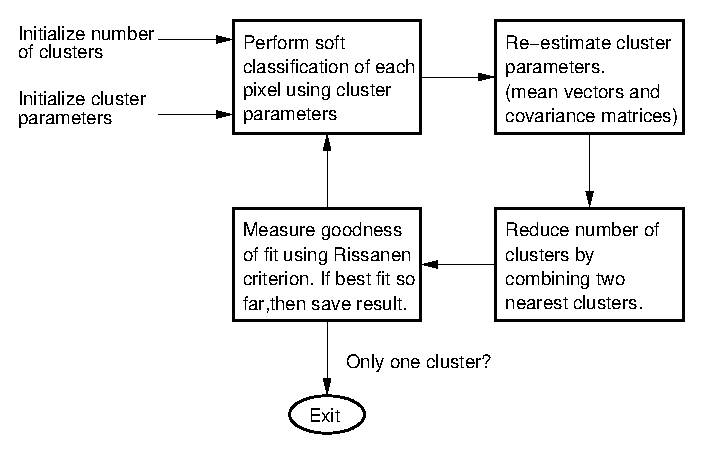
\includegraphics[width=4.5in]{fig3a.eps}}
\caption{This figure shows the basic operations performed in the
Cluster algorithm. At each step, the cluster parameters are saved
if they are the best observed so far. The final answer is the 
clustering that minimizes the goodness-of-fit measure.}
\label{fig:SigSet_flow_dia}
\end{figure}


\begin{figure}
\centerline{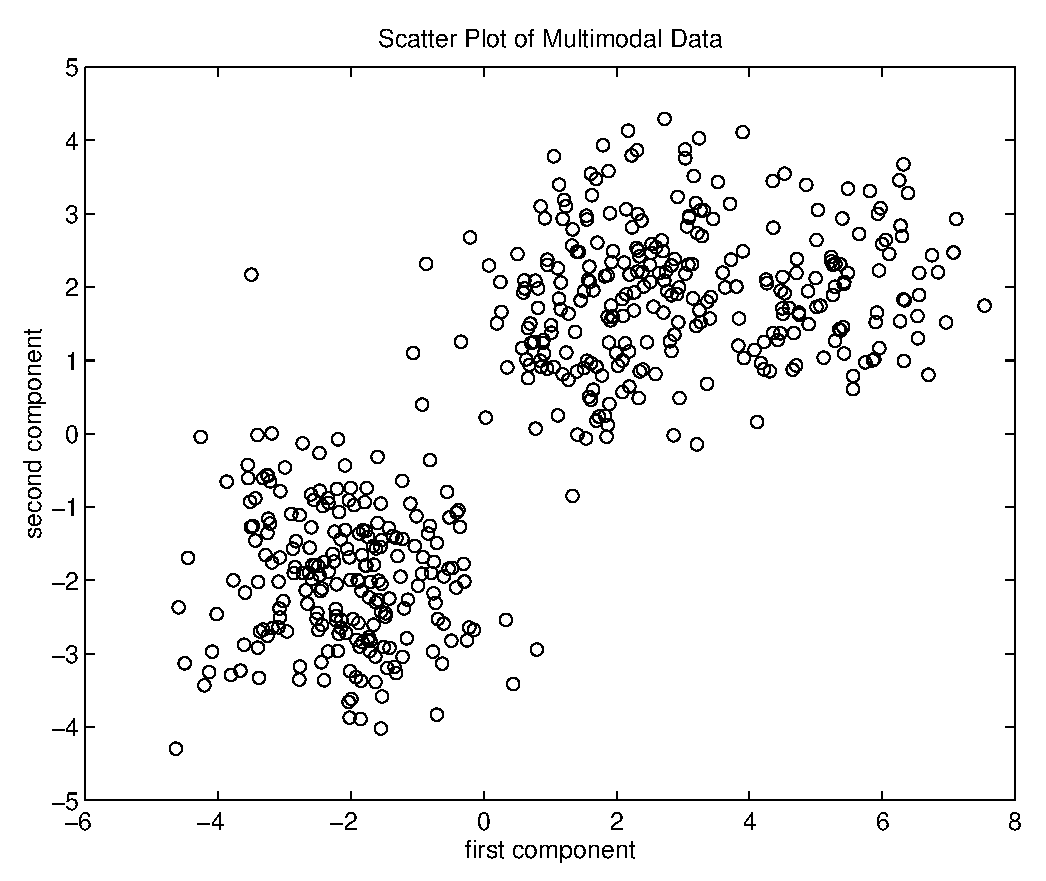
\includegraphics[width=4in]{scat_plot.eps}}
\caption{This figure shows a scatter plot generated using
random samples from a mixture model. The parameters of the 
mixture model are shown in Table~\ref{tbl:mix_params}.}
\label{fig:SigSet_scat_plot}
\end{figure}


\begin{table}
\centerline{
\begin{tabular}{|c|c|c|c|}\hline
 &parameter & true value & estimated value \\ \hline \hline
Cluster 1 & $\pi_1$ & 0.4 & 0.385141\\ \cline{2-4}
 & $\mu_1$ & [2.0 2.0] & [1.968770 1.908531] \\ \cline{2-4}
 & $R_1$ & $\left[ \begin{array}{cc}  1& 0.1\\ 0.1& 1 \end{array} \right]$ 
& $\left[ \begin{array}{cc}  1.089314 & 0.291036 \\ 0.291036 & 1.034361 \end{array} \right]$ \\ \hline
Cluster 2 & $\pi_2$ & 0.4 & 0.433581  \\ \cline{2-4}
 & $\mu_2$ & [-2.0 -2.0] & [-2.096070 --1.960741] \\ \cline{2-4}
 & $R_2$ & $ \left[ \begin{array}{cc}  1& -0.1\\ -0.1& 1 \end{array} \right]$ 
& $\left[ \begin{array}{cc}  1.089534 & -0.091958 \\ -0.091958 & 0.928903 \end{array} \right]$ \\ \hline
Cluster 3 & $\pi_3$ & 0.2 & 0.181277 \\ \cline{2-4}
 & $\mu_3$ & [5.5 2.0] & [5.333640 1.904941] \\ \cline{2-4}
 & $R_2$ & $ \left[ \begin{array}{cc}  1& 0.2\\ 0.2& 0.5 \end{array} \right]$ 
& $\left[ \begin{array}{cc}  0.870289 & 0.188515 \\ 0.188515 & 0.578056 \end{array} \right]$ \\ \hline
\end{tabular}}
\caption{Table showing the true and estimated parameters for
the samples shown in Fig~\ref{fig:SigSet_scat_plot}. 
Notice that the order of the model, $L=3$, is correctly estimated.
Each cluster is parameterized by its
relative proportion, $\pi_i$, its mean, $\mu_i$, and its covariance, $R_i$.}
\label{tbl:mix_params}
\end{table}


\begin{figure}
\centerline{\includegraphics[angle=-90]{ex1_mixture.ps}}
\caption{Estimated mixture probability density function.}
\label{fig:mix_pdf}
\end{figure}


\begin{figure}
\begin{center}
\parbox{5in}{\small
\noindent
Start clustering class 0\newline
Warning: Removed a singular subsignature; number 13; 19 remain\newline
Subclasses = 19; Rissanen = 2219.733222; Combining Subclasses (17,18)\newline
Subclasses = 18; Rissanen = 2198.894739; Combining Subclasses (12,13)\newline
Subclasses = 17; Rissanen = 2177.672102; Combining Subclasses (6,10)\newline
Subclasses = 16; Rissanen = 2157.009854; Combining Subclasses (7,10)\newline
Subclasses = 15; Rissanen = 2136.229106; Combining Subclasses (6,11)\newline
Subclasses = 14; Rissanen = 2116.872794; Combining Subclasses (0,7)\newline
Subclasses = 13; Rissanen = 2098.591172; Combining Subclasses (8,12)\newline
Subclasses = 12; Rissanen = 2079.471212; Combining Subclasses (5,7)\newline
Subclasses = 11; Rissanen = 2064.374351; Combining Subclasses (6,10)\newline
Subclasses = 10; Rissanen = 2050.283018; Combining Subclasses (2,4)\newline
Subclasses = 9; Rissanen = 2034.722833; Combining Subclasses (0,8)\newline
Subclasses = 8; Rissanen = 2018.317428; Combining Subclasses (2,7)\newline
Subclasses = 7; Rissanen = 2000.510965; Combining Subclasses (1,6)\newline
Subclasses = 6; Rissanen = 1984.862735; Combining Subclasses (3,4)\newline
Subclasses = 5; Rissanen = 1972.446690; Combining Subclasses (1,3)\newline
Subclasses = 4; Rissanen = 1956.088972; Combining Subclasses (0,3)\newline
Subclasses = 3; Rissanen = 1939.444535; Combining Subclasses (0,2)\newline
Subclasses = 2; Rissanen = 1949.218131; Combining Subclasses (0,1)\newline
Subclasses = 1; Rissanen = 2130.086314;\newline
}
\end{center}
\caption{This figure shows output of the Cluster program for the example data
set shown in Fig~\ref{fig:SigSet_scat_plot}. Notice that the minimum of the Rissanen
criteria occurs at the correct number of clusters (i.e. Subclasses = 3). }
\label{fig:SigSet_output}
\end{figure}













\clearpage
\newpage

\section{Program Manual Pages}
\label{sec:C_manual}


\begin{description}
\item {\bf clust}

This program is used to estimate the parameters
of a Gaussian mixture model.
It also estimates the number of clusters using 
the MDL criteria of Rissenen.

\item SYNOPSIS
\begin{verbatim}
clust #_subclasses info_file output_params [option1 option2]

    #_subclasses - initial number of clusters for each class

    info_file - name of file which contains the following information:
      <# of classes>
      <data vector length>
      <class 1 data file name> <# of data vectors in class 1>
      <class 2 data file name> <# of data vectors in class 2>
                     .                        .
                     .                        .
                     .                        .
      <last class data file name> <# of data vectors in last class>

    output_params - name of file containing output cluster parameters

    option1 - (optional) controls clustering model
      full - (default) use full convariance matrices
      diag - use diagonal convariance matrices

    option2 - (optional) controls number of clusters
      0 - (default) estimate number of clusters
      n - use n clusters in mixture model with n<#_subclasses
\end{verbatim}

\begin{description}

\item {\bf \#\_subclasses} - 
This is a number that specifies
the initial number of subclasses used to cluster the data.
The algorithm will automatically estimate the true number
of subclasses for each class being modeled.
However, it is good to start with an initial number of classes
with is about 2-3 time the number of classes estimated by the algorithm.

\item {\bf info\_file} - 
The program ``clust'' requires an ``info\_file'' that 
specifies a file name, $<$class k data file name$>$,
for each of the classes being modeled. 
Each file $<$class k data file name$>$ contains a list
of  $<$\# of data vectors in class k$>$ data vectors in ASCII
floating point format. Each data vector is
of length $<$data vector length$>$ and is on a single
line of the file.
Each vector is represents the components of the 
vector valued image at a single pixel and from a single
class k.

\item {\bf output\_params\_file} - 
An ASCII file which contains the 
parameters for the Gaussian mixture model used for each class.

\item {\bf option1} -  
An optional parameter value that controls the model used for
the Gaussian mixture. 
If the option is set to ``full'' than a full covariance matrix
is estimated for each subcluster.
This is the default assumption if no option is specified.
If the option is set to ``diag'' than a diagonal covariance matrix
is estimated for each subcluster.
This is equivalent to assuming that the components of each
subcluster are independent with different variances.

\item {\bf option2} -
An optional parameter value that controls the number of final clusters.
The default value of 0 indicates that the number of clusters should
be automatically estimated.

\end{description}



 \item DESCRIPTION

The {\em clust} program is used to determine the parameters
of a Gaussian mixture distribution.
The parameters may be estimated from a series of data
vectors corresponding to training samples for each 
class.
The mixture class parameters are stored as a class signature
which can be used 
for subsequent applications such as segmentation.

The {\em clust} program estimates both the number
of distinct subclasses in each class, 
and the spectral mean and covariance for each subclass.
The number of subclasses is estimated using 
Rissanen's minimum description length (MDL) criteria \cite{Ri83}.
This criteria attempts to determine the number of subclasses
which ``best'' describe the data.
The approximate maximum likelihood estimates
of the mean and covariance of the subclasses are computed using
the expectation maximization (EM) algorithm \cite{DeLaRu77,ReWa84}.
Refer to Appendix \ref{sec:parameter_est} for a detailed
derivation of the algorithm under the assumption that
the ``full'' option is used. 
The ``diag'' option is a straightforward modification
of this case.

\end{description}






\newpage
\section{Example Parameter File} 
\label{sec:params_file}


Figure \ref{fig:params_file}
is an annotated example of a parameter file which
is output from the {\em clust} program.
The subroutines read\_sig.c and write\_sig.c will 
read and write these parameters from the SigSet data structure
defined in the file sig.h.

Below is an example of a parameter file.
The original application for this clustering algorithm
was multispectral image segmentation; 
so the terminology used in the parameter file
reflects this application domain.
Notice that data sets are referred to as classes,
and components of the mixture distribution are referred
to as subclasses.

For this example, there are mixture models generated
for two sets of sample vectors.
Each set contained two dimenional sample vectors.
The first class is a simple multivariate
Gaussian distribution with a single cluster or subclass. 
The second class 
is a second order mixture with two clusters or subclasses. 



\begin{figure}
{\small
\begin{center}
\begin{minipage}{5in}
\hrulefill
\begin{verbatim}
title: Data_set_name
nbands: 2     /* number of dimensions to sample vectors */ 
class:        /* begin specification  for first data set*/
 classnum: 0  /* data set number 0 */
 classtitle:  /* data set title (optional) */
 classtype: 0 /* data set type (optional) */
 npixels: 0   /* number of sample vectors (optional) */
 subclass:    /* begin subclass specification */
  pi: 1.0     /* relative weight of subclass component */
  means: 127.0 128.0   /* vector of mean values */
  covar:               /* covariance matrix */
    64.0 0.0
    0.0  32.0
 endsubclass: /* end subclass specification */
endclass:     /* end class specification */
class:        /* begin class specification */
 classnum: 1  /* data set number 1 */
 classtitle:  /* data set title (optional) */
 classtype: 0 /* data set type (optional) */
 npixels: 0   /* number of sample vectors (optional) */
 subclass:    /* begin subclass specification */
  pi: 0.25    /* relative weight of subclass component */
  means: 32.0 32.0     /* vector of mean values */
  covar:               /* covariance matrix */
    100.0 2.0
    2.0   100.0
 endsubclass: /* end subclass specification */
 subclass:    /* begin subclass specification */
  pi: 0.75    /* relative weight of subclass component */
  means: 64.0 64.0     /* vector of mean values */
  covar:               /* covariance matrix */
    50.0 0.0
    0.0   25.0
 endsubclass: /* end subclass specification */
endclass:     /* end subclass specification */
\end{verbatim} 
\hrulefill
\end{minipage}
\end{center}
}
\caption{An example of a params file required
to specify two Gaussian mixture models.
Each mixture model is estimated from a distinct set 
of sample vectors.}
\label{fig:params_file}
\end{figure}


\newpage
\appendix



\section{Appendix: Parameter Estimation for Gaussian Mixture Models} 
\label{sec:parameter_est}

It is often desirable to model distributions
that are composed of distinct subclasses or clusters.
For example, a pixel in a image might behave differently
if it comes from an edge rather than a smooth region.
Therefore the aggregate behavior is likely to be a mixture
of the two distinct behaviors.
The objective of mixture distributions is to form a probabilistic
model composed of a number of component subclasses.
Each subclass is than characterized by a set of parameters
describing the mean and variation of the spectral components.

In order to estimate the parameters of a Gaussian mixture,
it is necessary to determine the
number of subclasses and the parameters of each subclasses.
This can be done by using a representative sample
of training data and estimating the number
of subclasses and their parameters from this data.

Specifically, let $Y$ be an $M$ dimensional random vector 
to be modeled using a Gaussian mixture distribution.
Let us assume that this model has $K$ subclasses.
The the following parameters are required to completely specify 
the $k^{th}$ subclass.
\begin{itemize}
\item[$\pi_k$] - the probability that a pixel has subclass $k$.
\item[$\mu_k$] - the $M$ dimensional spectral mean vector for subclass $k$.
\item[$R_k$] - the $M\times M$ spectral covariance matrix for subclass $k$.
\end{itemize}
Furthermore, let $K$ denote the number of subclasses,
then we use the notation $\pi$, $\mu$, and $R$ to
denote the parameter sets $\{\pi_k\}_{k=1}^K$, $\{\mu_k\}_{k=1}^K$, 
and $\{R_k\}_{k=1}^K$.
The complete set of parameters
for the information class
are then given by $K$ and $\theta = (\pi,\mu,R)$.
Notice that the parameters are constrained in a variety
of ways. 
In particular, $K$ must be an integer greater than 0,
$\pi_k\geq 0$ with $\sum_k \pi_k = 1$, 
and $det(R)\geq \epsilon$ where $\epsilon$ may be chosen depending
on the application.
We will denote the set of admissible $\theta$ for a $K^{th}$ order model 
by $\Omega^{(K)}$.

Let $Y_1,Y_2,\cdots,Y_N$ be $N$ multispectral pixels
sampled from the information class of interest.
Furthermore, assume that for each pixel $Y_i$
the subclass of that pixel is given by the random variable $X_n$
Of course, $X_n$ is usually not known, but it will be useful
for analyzing the problem.
Then assuming that each subclass has
a multivariate Gaussian distribution,
the probability density function for the pixel $Y_n$
given that $X_n=k$ is given by
$$
p_{y_n|x_n}(y_n|k,\theta) = \frac{1}{(2\pi)^{M/2}} \left| R_k \right|^{-1/2}
\exp \left\{ -\frac{1}{2} (y_n-\mu_k)^t  R_k^{-1} (y_n-\mu_k) \right\} \ .
$$
However, we do not know the subclass $X_n$ of each sample, so to compute
the density function of $Y_n$ given the parameter $\theta$ we must
apply the definition of conditional probability and sum over $k$.
$$
p_{y_n}( y_n |\theta ) = \sum_{k=1}^K p_{y_n|x_n}(y_n | k,\theta) \pi_k
$$
The log of the probability of the entire sequence $Y = \{Y_n\}_{n=1}^N$
is then given by
\begin{equation}
\log p_y( y |K,\theta ) = \sum_{n=1}^N \log \left( \sum_{k=1}^K
p_{y_n|x_n}(y_n | k,\theta) \pi_k \right) \ .
\label{eq:log_like}
\end{equation}

The objective is then to estimate the parameters
$K$ and $\theta \in \Omega^{(K)}$.
The maximum likelihood (ML) estimate is a commonly
used estimate with many desirable properties.
It is given by
$$
\hat{\theta}_{ML} = \arg \max_{\theta\in \Omega^{(K)}} \log p_y( y |K,\theta )
$$
Unfortunately, the ML estimate of $K$ is not well defined
because the likelihood may always be made better by choosing
a large number of subclusters.
Intuitively, the log likelihood may always be increased
by adding more subclasses since more subclasses may be
used to more accurately fit the data.

This problem of estimating the order of a model 
is known as order identification, and has been
studied by a variety of researchers.
Methods for estimating model order generally tend to require the addition
of a penalty term in the log likelihood to account
for the over-fitting of high order models.
One of the earliest approaches to order identification
was suggested by Akaike \cite{AK74},
and requires the minimization of the so called AIC
information criteria.
The AIC criterion is given by
$$
AIC(K,\theta) = -2\log p_y( y |K,\theta ) +2 L
$$
where $L$ is the number of continuously
valued real numbers required to specify the parameter $\theta$.
In this application,
$$
L =  K\left(1 + M + \frac{(M+1)M}{2}\right) - 1 \ .
$$
However, an important disadvantage of the AIC criteria
for a number of problems is that the AIC does not
lead to a consistent estimator \cite{Ka80}.
This means that as the number of observations tends to infinity,
the estimated value for $K$ does not converge to the true
value. 

Alternatively, another criterion was suggested by Rissanen \cite{Ri83}
called the minimum description length (MDL) estimator.
This estimator works by attempting to find the model order
which minimizes the number of bits that would be required to code
both the data samples $y_n$ and the parameter vector $\theta$.
While a direct implementation of the MDL estimator may depend on the
particular coding method used, Rissanen develop an approximate expression
for the estimate based on some assumptions and the minimization
of the expression
$$
MDL(K,\theta) = -\log p_y( y |K,\theta ) +\frac{1}{2} L \log (NM) \ .
$$
Notice that the major difference between the AIC and MDL criteria
is the dependence of the penalty term on the 
total number of data values $NM$. 
In practice, this is important since otherwise more data will tend to result
in over fitting of the model.
In fact, it has been shown that for a large number
of problems, the MDL criteria is a consistent estimator of model order \cite{Ka82,WaKa85}.
Unfortunately, the estimation of model order for mixture models
does not fall into the class of problems for which the MDL criteria
is known to be consistent.
This is due to the fact that the solution to the mixture model problem
always falls on a boundary of the constraint space,
so the normal results on the asymptotic distribution of the ML estimate
are no longer valid.
An alternative method for order identification which is known to be consistent
for mixture models is presented in \cite{ReWa84}.
However, this method is  computationally expensive  
when the dimensionality of the data is high.

Our objective will be to minimize the MDL criterion
given by
\begin{equation}
MDL(K,\theta) = -\sum_{n=1}^N \log \left( \sum_{i=1}^K
p_{y_n|x_n}(y_n | k,\theta) \pi_k \right)
+\frac{1}{2} L \log (NM)  \ .
\label{eq:MDL}
\end{equation}
Direct minimization of $MDL(\theta)$ is difficult for a number
of reasons.
First, the logarithm term makes direct optimization with
$\pi$, $\mu$, and $R$ difficult.
Second, minimization with respect to $K$ is complex since
for each value of $K$ a complete minimization with respect
to $\pi$, $\mu$, and $R$ is required.
If the subclass of each pixel, $X_n$, where known, then the estimation
of $\pi$, $\mu$, and $R$ would be quite simple.
Unfortunately, $X_n$ is not available. 
However, the expectation-maximization (EM) algorithm has been developed
to address exactly this type 
of ``incomplete'' data problem \cite{BaPeSoWe70,DeLaRu77}.

Intuitively, the EM algorithm works 
by first classifying the pixels $Y_n$ according
to their subclass,
and then re-estimating the subclass parameters based on this
approximate classification.
An essential point is that instead of the membership to each subclass
being deterministic,
the membership is represented using a ``soft'' probability.
The process is started by assuming the the true parameter
is given by $\theta^{(i)}$.
We index $\theta^{(i)}$ by $i$ because ultimately
the EM algorithm will result in a iterative procedure
for improving the MDL criterion.
The probability that pixel $y_n$ belongs to subclass $k$ may
then be computed using Bayes rule.
\begin{eqnarray*}
p_{x_n|y_n} (k|y_n,\theta^{(i)}) = 
\frac{p_{y_n|x_n} (y_n|k,\theta^{(i)}) \pi_k}
     {\sum_{l=1}^K p_{y_n|x_n} (y_n|l,\theta^{(i)}) \pi_l} \ .
\end{eqnarray*}
Then using these ``soft'' subclass memberships we will
then compute
new spectral mean and covariance estimates for each subclass.
We will denote these new estimates 
by $\bar{\pi}_k$, $\bar{\mu}_k$ and $\bar{R}_k$
where
\begin{eqnarray}
\label{eq:bar_values1}
\bar{N}_k &=& \sum_{n=1}^N p_{x_n|y_n} (k|y_n,\theta^{(i)}) \\
\label{eq:bar_values2}
\bar{\pi}_k &=& \frac{ \bar{N}_k }{N}\\
\label{eq:bar_values3}
\bar{\mu}_k &=& \frac{1}{\bar{N}_k}\sum_{n=1}^N y_n 
                p_{x_n|y_n} (k|y_n,\theta^{(i)}) \\
\label{eq:bar_values4}
\bar{R}_k &=& \frac{1}{\bar{N}_k}\sum_{n=1}^N 
(y_n-\bar{\mu}_k)(y_n-\bar{\mu}_k)^t p_{x_n|y_n} (k|y_n,\theta^{(i)})
\end{eqnarray}

In order to formally derive the EM algorithm update equations,
we must first compute the following function
$$
Q(\theta;\theta^{(i)}) 
= E\left[  \log p_{y,x}(y,X|\theta) | Y=y, \theta^{(i)} \right]
- \frac{1}{2} L \log (NM)
$$
where $Y$ and $X$ are the sets of random variables 
$\{Y_n\}_{n=1}^N$ and $\{X_n\}_{n=1}^N$ respectively,
and $y$ and $x$ are realizations of these random objects.
The fundamental result of the EM algorithm
which is proven in \cite{BaPeSoWe70} is that for all $\theta$
$$
MDL(K,\theta) - MDL(K,\theta^{(i)}) 
<
Q( \theta^{(i)}; \theta^{(i)}) - Q(\theta; \theta^{(i)}) \ .
$$
This results in a useful optimization method since 
any value of $\theta$ that increases the value of $Q(\theta; \theta^{(i)})$
is guarrenteed to reduce the MDL criteria.
The objective of the EM algorithm is therefore to iteratively
optimize with respect to $\theta$ until a local minimum
of the $MDL$ function is reached.

In order to derive expressions for the EM updates,
we first compute a more explicit form 
for the function $Q(\theta; \theta^{(i)})$.
The $Q$ function may be expressed in the following
form by substituting in for $\log p_{y,x}(y,x|\theta)$ and simplifying.
\begin{eqnarray*}
\lefteqn{ Q(\theta;\theta^{(i)}) = } \\
& & \sum_{k=1}^K \bar{N}_k \left\{
-\frac{1}{2} trace[\bar{R}_k R_k^{-1} ]
-\frac{1}{2} (\bar{\mu}_k -\mu_k)^t R_k^{-1}(\bar{\mu}_k -\mu_k)
-\frac{M}{2} \log(2\pi) 
-\frac{1}{2} \log(|R_k|) 
+\log(\pi_k) \right\} \\
& & - \frac{1}{2} L \log (NM)
\end{eqnarray*}
where $\bar{N}_k$, $\bar{\mu}_k$, and $\bar{R}_k$ are as 
given in (\ref{eq:bar_values1}), (\ref{eq:bar_values2}), and (\ref{eq:bar_values3}).

We will first consider the maximization of $Q(\theta; \theta^{(i)})$
with respect to $\theta\in \Omega^{(K)}$.
This maximization of $Q$ may be done using Lagrange multipliers
and results in the update equations
\begin{eqnarray}
\nonumber
(\pi^{(i+1)},\mu^{(i+1)},R^{(i+1)}) 
&=&  \arg \max_{ (\pi,\mu,R)\in \Omega^{(K)} }
Q(\theta;\theta^{(i)}) \\
&=& (\bar{\pi},\bar{\mu},\bar{R}) 
\label{eq:EM1_update}
\end{eqnarray}
where $(\bar{\pi},\bar{\mu},\bar{R})$ may be computed using 
(\ref{eq:bar_values1}), (\ref{eq:bar_values2}), (\ref{eq:bar_values3}), and (\ref{eq:bar_values4}).

While (\ref{eq:EM1_update}) shows how to update the parameter $\theta$,
it does not show how to change the model order $K$.
Our approach will be to start with a large number of clusters,
and then sequentially decrement the value of $K$.
For each value of $K$, we will apply the EM update of (\ref{eq:EM1_update})
until we converge to a local minimum of the MDL functional.
After we have done this for each value of $K$, we may simply
select the value of $K$ and corresponding parameters
that resulted in the smallest value of the MDL criteria.

The question remains of how to decrement the number of clusters
from $K$ to $K-1$. 
We will do this by merging two clusters to form a single cluster.
One way to effectively reduce the order 
of a model is to constrain the parameters
of two subclasses to be equal.
For example, two subclasses, $l$ and $m$, may be effectively
``merged'' in a single subclass by constraining their mean and covariance
parameters to be equal.
\begin{eqnarray}
\label{eq:constraint}
\mu_l &=&  \mu_m = \mu_{(l,m)} \\
\nonumber
R_l &=&  R_m = R_{(l,m)} 
\end{eqnarray}
Here $\mu_{(l,m)}$ and $R_{(l,m)}$ denote the mean and covariance
of the new subclass,
and we assume that the values of $\pi_l$ and $\pi_m$ remain unchanged
for the two clusters being merged.
We denote this modified parameter vector by $\theta_{(l,m)} \in \Omega^{(K)}$.
Notice that since 
$\theta_{(l,m)}$ specifies the parameters for $K$ clusters,
it is a member of $\Omega^{(K)}$, 
but that two of these clusters (e.g. clusters $l$ and $m$)
have identical cluster means and covariance.
Alternatively, we use the notation $\theta_{(l,m)^-} \in \Omega^{(K-1)}$
to denote the parameters for the $K-1$ distinct clusters
in $\theta_{(l,m)}$.
More specifically, the two clusters $l$ and $m$ are specified
as a single cluster $(l,m)$ with mean and covariance 
as given in (\ref{eq:constraint}), and
prior probability given by
\begin{equation}
\pi_{(l,m)} = \pi_l+\pi_m \ .
\label{eq:newprior}
\end{equation}

Using these definitions for $\theta_{(l,m)}$ and $\theta_{(l,m)^-}$,
then the following relationship is results from inspection of (\ref{eq:MDL}).
$$
MDL(K-1,\theta_{(l,m)^-}) = MDL(K,\theta_{(l,m)}) 
+ \frac{1}{2} \left(1 + M + \frac{(M+1)M}{2}\right) \log (NM)  \ .
$$
The change in the MDL criteria is then given by
\begin{eqnarray*}
&& MDL(K-1,\theta_{(l,m)^-}) - MDL(K,\theta^{(i)}) \\
&=& MDL(K-1,\theta_{(l,m)^-}) - MDL(K,\theta_{(l,m)}) 
  + MDL(K,\theta_{(l,m)}) - MDL(K,\theta^{(i)})\\
&\leq&  - \frac{1}{2} \left(1 + M + \frac{(M+1)M}{2}\right) \log (NM)
  + Q(\theta^{(i)};\theta^{(i)}) - Q(\theta_{(l,m)};\theta^{(i)})\\
&\leq&  - \frac{1}{2} \left(1 + M + \frac{(M+1)M}{2}\right) \log (NM)\\
&& + Q(\theta^{(i)};\theta^{(i)}) - Q(\theta^*;\theta^{(i)}) 
  + Q(\theta^*;\theta^{(i)}) - Q(\theta^*_{(l,m)};\theta^{(i)})\ .
\end{eqnarray*}
where $\theta^*$ and $\theta^*_{(l,m)}$ are the unconstrained 
and constrained optima respectively.
The solution to the unconstrained optimization, $\theta^*$,
is given in equation (\ref{eq:EM1_update}).
We will assume that the EM algorithm has been run to convergence
for a fixed order $K$, so that $\theta^*=\theta^{(i)}$.
In this case, 
$$
Q(\theta^{(i)};\theta^{(i)}) - Q(\theta^*;\theta^{(i)}) = 0 \ .
$$
The value of $\theta^*_{(l,m)}$ is obtained 
by maximizing $Q(\theta_{(l,m)};\theta^{(i)})$
as a function of $\theta_{(l,m)}$ subject 
to the constraints of (\ref{eq:constraint}).
This constrained optimization results in the same values 
of $\pi^*_l=\bar{\pi}_l$ and $\pi^*_m=\bar{\pi}_m$
as in the unconstrained case, 
but the following new mean and covariance values.
\begin{eqnarray}
\label{eq:param_add2}
\mu_{(l,m)}^* &=& \frac{\bar{\pi}_l \bar{\mu}_l + \bar{\pi}_m \bar{\mu}_m}
             { \bar{\pi}_l + \bar{\pi}_m} \\
\label{eq:param_add3}
R_{(l,m)}^* &=& \frac{
\bar{\pi}_l \left( \bar{R}_l + (\bar{\mu_l} - \mu_{(l,m)}) (\bar{\mu_l} - \mu_{(l,m)})^t\right) 
+ \bar{\pi}_m \left( \bar{R}_m + (\bar{\mu_m} - \mu_{(l,m)}) (\bar{\mu_m} - \mu_{(l,m)})^t\right) 
}{ \bar{\pi}_l + \bar{\pi}_m} \ .
\end{eqnarray}
Here the $\bar{\pi}$, $\bar{\mu}$, and $\bar{R}$
are given by (\ref{eq:bar_values2}), (\ref{eq:bar_values3}), 
and (\ref{eq:bar_values4}),
and the remaining values of $\pi_k$, $\mu_k$, and $R_k$ are
unchanged from the unconstrained result.
Using (\ref{eq:param_add2}) and (\ref{eq:param_add3}), 
we may define a distance function with the form
\begin{eqnarray}
\nonumber
d(l,m) 
&=& Q(\theta^*;\theta^{(i)}) - Q(\theta^*_{(l,m)};\theta^{(i)})\\
\nonumber
&=& N \bar{\pi}_l \left\{ - \frac{M}{2} (1+\log(2\pi)) 
    -  \frac{1}{2} \log(|\bar{R}_l|) \right\}\\
\nonumber
& & + N \bar{\pi}_m \left\{ - \frac{M}{2} (1+\log(2\pi)) 
    -  \frac{1}{2} \log(|\bar{R}_m|) \right\}\\
\nonumber
& & - 2N \pi_{(l,m)} \left\{ - \frac{M}{2} (1+\log(2\pi)) 
    -  \frac{1}{2} \log(|R_{(l,m)}|) \right\} \\
\label{eq:distancefunction}
&=& \frac{N \bar{\pi}_l}{2} \log\left( \frac{|R_{(l,m)}|}{|\bar{R}_l|} \right)
 +  \frac{N \bar{\pi}_m}{2} \log\left( \frac{|R_{(l,m)}|}{|\bar{R}_m|} \right)
\end{eqnarray}
This distance function then serves as an upper bound on the
change in the MDL criteria.
\begin{eqnarray}
MDL(K-1,\theta_{(l,m)^-}) - MDL(K,\theta^{(i)})
\leq d(l,m) - \frac{1}{2} \left(1 + M + \frac{(M+1)M}{2}\right) \log (NM)  
\label{eq:MDLbound}
\end{eqnarray}

A few comments are in order.
The value of $d(l,m)$ is always positive.
This is clear from the form of (\ref{eq:distancefunction}).
In fact, reducing the model order should only reduce
the log likelihood of the observations since there are fewer
parameters to fit the data.
In general, this increase may be offset by the model order
term in (\ref{eq:MDLbound}) which is always negative.
However, since this term is independent of the choice of $l$
and $m$, it does not play a role
in selecting which clusters to merge.

With the function $d(l,m)$ precisely defined, it is now possible
to search over the set of all pairs, $(l,m)$, to find the
cluster pair which minimizes $d(l,m)$,
thereby minimizing an upper bound on the change in the MDL criteria.
\begin{eqnarray}
\label{eq:reduce_update}
(l^*,m^*) = \arg \min_{(l,m)} d(l,m) 
\end{eqnarray}
These two clusters are then merged.
The parameters of the merged cluster are computed using
(\ref{eq:newprior}) and (\ref{eq:param_add2}),
and the resulting parameter set $\theta_{l,m}^*$ 
is used as a initial condition for EM optimization
with $K-1$ clusters.

Before we can specify the final Cluster algorithm,
we must specify the initial choice 
of the parameter $\theta^{(1)}$ used with the largest number of clusters.
The initial choice of $\theta^{(1)}$ can be important
since the EM is only guaranteed to converge to a local minimum.
The initial number of clusters, $K_o$, is chosen by the user
subject to the constraint that the total number of parameters, 
$L<\frac{1}{2}MN$.
The initial subclass parameters are then chosen to be
\begin{eqnarray}
\label{eq:EM_init1}
\pi_k^{(1)} &=& \frac{1}{K_o} \\
\label{eq:EM_init2}
\mu_k^{(1)} &=& y_n \mbox{ where } n = \lfloor (k-1)(N-1)/(K_o-1) \rfloor +1\\
\label{eq:EM_init3}
R_k^{(1)} &=& \frac{1}{N} \sum_{n=1}^N y_n y_n^t
\end{eqnarray}
where $\lfloor \cdot \rfloor$ is the greatest smaller integer function.

The final Cluster algorithm is given in the following steps.
\begin{enumerate}
\item Initialize the class with a large number of subclasses, $K_o$.
\item Initialize $\theta^{(1)}$ using (\ref{eq:EM_init1}), (\ref{eq:EM_init2}) and (\ref{eq:EM_init3}). 
\item Apply the iterative EM algorithm (\ref{eq:EM1_update}) until the change in
$MDL(K,\theta)$ is less then $\epsilon$.
\item Record the parameter $\theta^{(K,i_{final})}$, and value $MDL(K,\theta^{(K,i_{final})})$.
\item If the number of subclasses is greater than 1, 
apply equation (\ref{eq:reduce_update}) to reduce the number of clusters,
set $K\leftarrow K-1$, and go back to step 3.
\item Choose the value $K^*$ and parameters $\theta^{(K^*,i_{final})}$ 
which minimize the value of MDL.
\end{enumerate}

In step 3, the value of $\epsilon$ is chosen to be
$$
\epsilon = \frac{1}{100} \left( 1+M+\frac{(M+1)M}{2} \right) \log (NM) \ . 
$$




\begin{thebibliography}{99}

%\bibitem{BoSh92}
%C. Bouman and M. Shapiro,
%``Multispectral Image Segmentation  using  a Multiscale Image Model,''
%{\em Proc. of IEEE Int'l Conf. on Acoust.,  Speech  and  Sig.  Proc.,}
%pp. III-565  -  III-568,  San  Francisco, California, March 23-26, 1992.

%\bibitem{BoSh94}
%C. A. Bouman and M. Shapiro, 
%``A Multiscale Random Field Model for Bayesian Image Segmentation,''
%{\em IEEE Trans. on Image Processing,}
%vol. 3, no. 2, pp. 162-177, March 1994.

%\bibitem{McEn95}
%J. D. McCauley and B. A. Engel, 
%``Comparison of Scene Segmentation SMAP, ECHO, and Maximum Likelihood''
%{\em IEEE Trans. on Geoscience and Remote Sensing,}
%vol. 33, no. 6, pp. 1313-1316, November 1995.

\bibitem{AK74}
H. Akaike, ``A New Look at the Statistical Model Identification'',
{\em IEEE Trans. Automat. Contr.,}
vol. AC-19, pp. 716-723, December 1974.

\bibitem{Ri83}
J. Rissanen,
``A Universal Prior for Integers and Estimation by Minimum
Description Length,''
{\em Annals of Statistics,}
vol. 11, no. 2, pp. 417-431, 1983.

\bibitem{Ka80}
R. L. Kashyap,
``Inconsistency of the AIC Rule for Estimating the Order of Autoregressive Models,''
{\em IEEE Trans. Automat. Contr.,}
vol. AC-25, no. 5, Oct. 1980.

\bibitem{Ka82}
R. L. Kashyap,
``Optimal Choice of AR and MA Parts in Autoregressive Moving Average Models,''
{\em IEEE Trans. on Pattern Analysis and Machine Intelligence,}
vol. PAMI-4, no. 2, pp. 99-104, March 1982.

\bibitem{WaKa85}
M. Wax and T. Kailath,
``Detection of Signals by Information Theoretic Criteria,''
{\em IEEE Trans. on Acoustics, Speech, and Signal Processing,}
vol. ASSP-33, no. 2, pp. 387-392, April 1985.

\bibitem{ReWa84}
E. Redner and H. Walker, ``Mixture Densities, Maximum Likelihood and
the EM Algorithm,'' {\em SIAM Review,} vol. 26, no. 2, April 1984.

\bibitem{BaPeSoWe70}
L. Baum, T. Petrie, G. Soules, N. Weiss,
``A Maximization Technique Occurring in the Statistical Analysis
of Probabilistic Functions of Markov Chains,''
{\em Ann. Math. Statistics,} vol. 41, no. 1, pp. 164-171, 1970.

\bibitem{DeLaRu77}
A. Dempster, N. Laird and D. Rubin,
``Maximum Likelihood from Incomplete Data via the EM Algorithm,''
{\em J. Roy. Statist. Soc. B,} vol. 39, no. 1, pp. 1-38, 1977.


\end{thebibliography}




\end{document}

